\documentclass[preprint,12pt]{elsarticle}


% Packages
\usepackage{amssymb}
\usepackage{amsmath} % align
\usepackage{color}
\usepackage{graphicx}
\usepackage{subfigure}

\journal{Pattern Recognition}

\begin{document}

\newcommand{\cpos}{\text{\scriptsize{{\it POS}}}}
\newcommand{\cneg}{\text{\scriptsize{{\it NEG}}}}


\begin{frontmatter}

\title{A bag-to-class divergence approach to multiple-instance learning}


\begin{abstract}

A concise and factual abstract is required (maximum length 150 words). The abstract should state briefly the purpose of the research, the methods used, the principal results and major conclusions. An abstract is often presented separate from the article, so it must be able to stand alone.

\end{abstract}

\begin{keyword}
%Immediately after the abstract, provide a maximum of five to ten keywords, using American spelling and avoiding general and plural terms and multiple concepts (avoid, for example, 'and', 'of'). Be sparing with abbreviations: only abbreviations firmly established in the field may be eligible. These Keywords will be used for indexing purposes.

Multi-instance \sep Multiple-instance \sep Query-to-model \sep Object-to-class \sep Divergence \sep Dissimilarity \sep Classification \sep Uncertain object \sep Image analysis \sep Prototype \sep Template matching \sep
Multiple-instance learning \sep bag-to-class
\end{keyword}

\end{frontmatter}

\clearpage

\section{Introduction} \label{sec:Introduction} 
\subsection{History} 

% Janitor story

Multiple-instance learning (MIL) is a form of supervised learning where each object consists of several observations.
The observations themselves are not labelled, but the objects are.  
An object is referred to as {\it bag} in the MIL context, and the individual observations within the bag are referred to as {\it instances}.
In binary MIL, the classes are referred to as {\it positive} and {\it negative}. 
Image classification is a typical example of MIL. 
Each image (bag) consists of a number of pixels (instances).
An image in the training set is labelled 'positive' if it contains a certain material or body of interest, e.g. tumour tissue, and 'negative' if the material is absent. 
However, the location of the material within the image is unknown, and hence, the individual pixels are not labelled. 
A positive image contains pixels both from the tumour and from normal tissue, whereas a negative image contains only pixels from normal tissue. 
The task is to train a classifier using the pixels values, but with information only on image level. 

The term multiple instance learning was introduced by {\color{green} Dietterich et at (1997)}. 
The musk data was introduced, where some molecules will give a musk odour (positive class), others will not (negative class). 
Each molecule has different shapes, and only certain shapes will give the musky smell. 
Hence, each molecule is a bag, and the various shapes are its instances. 
The assumption is that if a bag contains at least one positive instance, the bag is positive, whereas negative bags contains only negative instances. 
This is referred to as the standard assumption. 
The main task is to identify the positive instances. 
If this is done successfully, classification is straightforward.

Since then, the MIL field has developed and expanded. 
Most notably, the strict assumption of Dietterich has been relaxed and replaced by other assumptions. 
MIL was introduced as a binary classification problem, but is applicable also in multiple classification, regression and clustering. 
This article will stick to the binary classification, but will go beyond the standard assumption. 

A relaxed assumption for the image example can be that the pixel intensity $x_i$ measured in tumour tissue is above a certain threshold $T_{tissue}$ (positive instance).  
In normal tissue, the intensity can also be above this threshold, but it will be fewer pixels. 
Hence, both positive and negative bags contain positive instances, but the assumption is that positive bags contains a larger number of positive instances than negative bags. 

{\color{green} Weidmann et al (2003)} introduced a hierarchy of assumptions, with the standard assumption as the least general. 
In the review article of {\color{green} Foulds and Frank (2010)}, the Weidmann hierarchy is part of a more extensive taxonomy for MIL assumptions, where also the data representations and similarity measures are taken into account. 

{\color{green} Amores (2013)} provides a different viewpoint and taxonomy, focusing on the type of information; instance-level or bag-level, and the representation of the information; explicitly or implicitly. 
Both Amores and Foulds and Frank categorise a range of previously proposed algorithm within their taxonomy, many of them whose assumption or information have not been explicitly stated by the authors. 
Amores and Foulds and Frank offer different and complementary analyses of the MI problem and its proposed algorithms, and touch upon many of the same obstacles and choices: 
\begin{itemize}
  \item Assumption
  \item Type of information (instance vs bag)
  \item Information representation (explicit vs implicit)
  \item Dissimilarity measures
  \item Prototypes/concepts
\end{itemize}

As the MI methodology has developed over the last few decades, the need for relaxed assumptions has arisen and has been incorporated in new methods and algorithms. 
As in all fields of research, there is no universal MI methodology that solves all problems the best. 
Using stricter assumptions is beneficial if the data meet them, but can be devastating if they are violated.
The problems to be solved are of different characteristics, and the methodology must be chosen accordingly. 

This paper offers an alternative viewpoint for MI classification: Hierarchical distribution and bag-to-class divergence. 
The hierarchical distribution describes the assumption of the instances in each bag, whereas the bag-to-class divergence offers a dissimilarity measure. 
The alternative viewpoint can be fitted into both Foulds and Frank's and Amores taxonomy, by adding and specifying properties. 

The rest of the article is organised as follows: 
Section {\color{blue} Assumption} describes the assumptions of the instances being observations from an underlying distribution. 
In addition, the assumptions regarding the distribution is made. 
Section {\color{blue} Bag-to-class dissimilarity} describes divergence functions as dissimilarity measures in MIL.
Section {\color{blue} Taxonomy} places the hierarchical distribution and the bag-to-class divergence approach within the taxonomies of Amores and Foulds and Frank.
Section {\color{blue} Simulations and real data} gives simulated and real data examples of the proposed MIL.
Section {\color{blue} Results} discusses the results from Simulations and real data.
Section {\color{blue} Discussion} gives an overall discussion regarding the introduced view on MIL and the proposed concept. 




\section{A probabilistic framework for MI problems} \label{sec:Probabilistic} 
The instances in a bag are most often treated as fixed points, but can also be viewed as observations of random variables with an (unknown) probability distribution. 
The probabilistic viewpoint is not an MI assumption by itself, but can be used as a tool to analyse the problem and choose the appropriate concept. 

For ease of notation, we will not use bold characters to denote vectors, as there is no need to distinguish between vectors and scalars in the following, and we will refer to random vectors as random variables.
The superscript $^+$ or $^-$ refers to the instance class, the subscript $_{pos}$ or $_{neg}$ refers to the class label of the bag. 

Let $X^+$ denote the random variable of a positive instance, and let $f^+(x|\theta_b^+)$ denote the pdf of the positive instances in bag $b$. 
Similarly, Let $X^-$ denote the random variable of a negative instance, and let $f^-(x|\theta_b^-)$ denote the pdf of the negative instances in bag $b$. 
Then, the pdf of bag $b$ is
\begin{align}
  f_b(x) = \pi^+_b f^+(x|\theta_b^+) + (1-\pi^+_b)f^-(x|\theta_b^-),
\end{align}
where $0 \leq \pi^+_b \leq 1$ denotes the proportion of positive instances in bag $b$. 

As an illustrative example, consider images of tissue with class label {\it tumour} (positive) or {\it normal} (negative). 
The image is the bag, and the pixels or image segments are its instances. 
The value of each pixel is then considered to be an observation from the underlying bag distribution. 
A pixel will belong to either tumour, with pdf $f^+(x|\theta_b^+)$, or normal tissue, $f^-(x|\theta_b^-)$, but the individual pixels are not labelled. 
In image $b$, a certain proportion are tumour pixels ($\pi^+_b$), the rest ($1-\pi^+_b$) are normal pixels.  
The pixels from tumour image $b$ has pdf
\begin{align}
  f_{b,pos}(x) = \pi^+_{b,pos} f^+(x|\theta_b^+) + (1-\pi^+_{b,pos})f^-(x|\theta_b^-).
\end{align}
Similarly, the pixels from a normal image $b'$ has pdf
\begin{align}
  f_{b',neg}(x) = \pi^+_{b',neg} f^+(x|\theta_{b'}^+) + (1-\pi^+_{b,neg})f^-(x|\theta_{b'}^-).
\end{align}
Since both tumour and normal tissue vary from image to image, we assume $\theta_b^+$ being an observation from the distribution $P(\Theta|\tau^+)$ and $\theta_b^-$ being an observation from the distribution $P(\Theta|\tau^-)$, where $\tau^+$ and $\tau^-$ are parameters. 
And since the tumour size varies, we also assume that $\pi^+_{b,pos}$ is an observation from $P(\Pi^+_{pos})$. 
Written as a hierarchical distribution: 
\begin{align}
  X_{pos}|\Theta & \sim P(X_{pos} | \Theta) \\
  \Theta|\mathcal{T} &  \sim P(\Theta|\mathcal{T}) \\
  \mathcal{T} & \sim \begin{cases}
    P(\mathcal{T} = \tau^+) = \Pi_{pos}^+\\
    P(\mathcal{T} = \tau^-)  = 1-\Pi_{pos}^+
  \end{cases} \\
  \Pi_{pos}^+ & \sim P(\Pi^+_{pos})
\end{align}
Similarly, for the normal images we have
\begin{align}
  X_{neg}|\Theta & \sim P(X_{neg} | \Theta) \\
  \Theta|\mathcal{T} &  \sim P(\Theta|\mathcal{T}) \\
  \mathcal{T} & \sim \begin{cases}
    P(\mathcal{T} = \tau^+) = \Pi_{neg}^+\\
    P(\mathcal{T} = \tau^-)  = 1-\Pi_{neg}^+
  \end{cases} \\
  \Pi_{neg}^+ & \sim P(\Pi^+_{neg})
\end{align}

The pdf of positive bags is then
\begin{align*}
  f_{pos}(x) = \pi_{pos}^+ \int_{\Theta|\tau^+} f^+(x|\theta)h(\theta|\tau^+) d\theta|\tau^+  +(1-\pi_{pos}^+) \int_{\Theta|\tau^-} f^-(x|\theta) h(\theta|\tau^-) d\theta|\tau^-, 
\end{align*}
where $\theta^+_b$ is the $b$th observation of the random variable $\theta$ with parameter $\tau^+$, and $\theta_b^-$ is the $b$th observation of the random variable $\theta$ with the parameter $\tau^-$.


\subsection{MI assumption in the probabilistic framework}
This is a general description of the origin of the instances, and does not imply any MI assumptions. 
Restrictions on the different levels of the hierarchical distribution will correlate to MI assumptions.
The standard MI assumption is then \\
(1) $P(\Pi^+_{neg} = 0) = 1$: No positive instances in a negative bag\\
(2) $0<\pi^+_{pos} \leq 1$: At least one positive instance in a positive bag\\
(3) $\mathcal{X}^+ \cap \mathcal{X}^- = \emptyset$ : No overlap between the set of possible positive values and possible negative values \\
The last assumption is generally not explicitly stated, but many algorithms are dedicated to finding $\mathcal{X}^+$, and thereafter use a concept that assumes (3). 

The count-based assumption is\\
(1) $t_{low,pos} < \pi^+_{pos} < t_{up,pos}$ \\
(2) $\mathcal{X}^+ \cap \mathcal{X}^- = \emptyset$ 

The count-based GMIL can be defined in the probabilistic setting by letting $\pi^+_{pos}$ be a vector with $k$ elements, and $\pi^+_{b,pos} f^+(x|\theta_b^+) = \sum_{k = 1}^K \pi^+_{b,pos,k} f^+_k(x|\theta_{b,k}^+)$, with the restrictions\\
(1) $\max \{\pi^+_{pos,k} == 0\} = r$ \\
(2) $\mathcal{X}^+_k$: defines {\it sufficiently close}. \\
(3) $\mathcal{X}^+_k \cap \mathcal{X}^- = \emptyset$ for all $k$ 

\subsection{Level of information in the probabilistic framework}
In the review article of Amores, MIL algorithms are categorised according to whether concepts are based on instance-level information or bag-level information. 
For the instance-level based concepts, the classifier is an aggregation of instance level scores, and any characteristic of the bags themselves are ignored. 
An example of this is the {\it collective} assumption in Foulds and Frank, where the concept is based on the (estimated) posterior class label of the instances: $P(c|b) = \frac{1}{n_b} \sum_{i = 1}^{n_b} Pr(c|x_i)$. 

The bag-level information is categorised into bag space and embedded space, where embedded space means that each bag is mapped to a single feature vector, and a single instance classifier is used. 
In the bag space, the classifiers are based on a dissimilarity measure (distances or kernel functions) comparing bags.

As with the MI assumptions, the probabilistic framework does not directly imply instance-level, bag-space or embedded-space. 
Since each bag is described as a pdf, it fits into the bag space. 
The probabilistic framework is applicable to instance-level information, as in the collective assumption. 
Embedded space can easily be use by estimating the parameters of the pdfs. 


% \section{Description} \label{sec:Description}
% Instances in a bag, $\mathbf{x}_i$, are observations from an underlying distribution. 
In the collective assumption, the instances of two bags belonging to the same class are (implicitly) assumed to be drawn from the same distribution.
We will generalise this assumption by a hierarchical approach: 
\begin{align}
  \mathbf{x}_i & \sim P(X|\mathbf{\Theta}_{b_k}) \\
  \mathbf{\Theta} & \sim P(\mathbf{\Theta}|\mathbf{\tau}_j), 
\end{align}
where $\mathbf{\tau}$ is a fixed parameter vector defined by the class. 

This could be a simple embedded approach, saying $D(\mathbf{\theta}, \mathbf{\tau})$, but instead the observations are used directly. 

How does the hierarchical assumption describe real-life bags?
If we go back to the tumour image example, we can assume that tumour pixels are drawn from the distribution $f(\mathbf{x}|\theta_{tum})$ and normal tissue pixels are drawn from the distribution $f(\mathbf{x}|\theta_{norm})$. Then, a pixel from an image containing a tumour will be drawn from the distribution 
\begin{align}
  f_{pix}(\mathbf{x}|\theta_{tum},\theta_{norm}, \pi_{tum}) = \pi_{tum}f(\mathbf{x}|\theta_{tum}) + (1-\pi_{tum})f(\mathbf{x}|, \theta_{norm})
\end{align}
where $0 < \pi_{tum} \leq 1$ is the proportion of the image occupied by the tumour.  
A pixel from an image not containing a tumour will be drawn from the same distribution, but with $\pi_{tum} = 0$.
In this simple example, the $\theta$'s are kept constant, but we can imagine without difficulty situations where the $\theta$'s will vary according to some distribution. 


% \section{Assumptions} \label{sec:Assumptions}
% A bag consists of several instances. 
An instance is an observation from an underlying distribution. Hence, we are making a {\it collective} assumption.
However, the classification does not simply follow the posterior probability of a bag belonging to a class. 
In the collective assumption, the choices/estimates are
the distribution:\\
\begin{align}
  P(X|\mathbf{\theta}_{b_i}), \, &i = 1, 2, \ldots, n_{bag} \\
  P(X|\mathbf{\theta}_{c_j}), \, & j = 1, 2, \ldots, n_{class}
\end{align}
a divergence: \\
\begin{align}
  & D(P(X|\mathbf{\theta}_{b_i}), P(X|\mathbf{\theta}_{c_j}))
\end{align}
and a classification 
\begin{align}
  \min_{\forall j} \{ D(b_i, c_j)\}
\end{align}

Following the taxonomy of Foulders and Franks and Amores, we have the following: \\
{ \bf Instance-level vs bag-level information:} 
The information is at bag-level. 
Amores also points out the drawbacks of instance-level information. \\
{\bf Implicit vs explicit information:} 
One method is to transform the multiple instances of a bag to a single vector, and the use single-instance learning. 
This could have been used with distribution information by estimating the a parameter vector. 
However, it is not suited in most occasions, because the knowledge about the distribution is too little. \\
{\bf Dissimilarity:} 
This is referred to as {\it distance}, but is not necessarily a distance function in the mathematical definition. 
This is a very influential choice. 
The previously proposed methods use bag-to-bag distance, but we will introduce the use of bag-to-class distance. 



\section{Probabilistic MI classifiers} \label{sec:Classifier}
As with all classification problems, if we knew the exact nature of the data, an optimal classifier could be chosen. 
Instead, we have to choose between very general assumptions that lead to sub-optimal classifiers, or stronger assumptions that ensure higher performance, but only if the assumptions are correct. 
There are three fundamental levels for MI problems:
(1) Choice of MI assumption \\
(2) Estimation \\
(3) Choice of classifier
These three steps are present both for deterministic and probabilistic viewpoint, and step (3) is closely linked to step (1) and (2). 
In the probabilistic framework, the choice of MI assumption can be stated as restrictions on the underlying pdfs. 
The pdfs that are used in classification of new bags have to be estimated based on the available bags with labels. 
Finally, the classifier can be chosen and trained based on the previous assumptions and choices. 

The most general MI assumption in the probabilistic framework is that $\tau^+ \neq \tau^-$ (the pdf of positive instances is different from the pdf of negative instances) and $\Pi_{pos}^+ \neq \Pi_{neg}^+$ (the distribution of the proportion of positive instances in a positive bag is different form that of positive instances in a negative bag). 

Accurate estimation the four levels of the Baye's hierarchy is out of reach for most problems. 
Therefore, we suggest to directly estimate the pdf of a bag with unknown label based on its instances, $\hat{f}_{bag}(x)$.
A dissimilarity measure can now be chosen to constitute the classifier. 

In Amores, all bag level classifiers are based on bag-to-bag dissimilarity measures. 
As pointed out by the author, this has the drawback that the number of comparisons that has to be made increases exponentially, and so the computational burden.
However, instance level algorithms suffer from inaccurate information (the true instance labels are not known), and the embedded space algorithms suffer from possible oversimplification. 

We therefore suggest a bag level classifier based on the bag-to-class dissimilarity. 
Hence, there are only two comparisons for each classification. 

Let $f_\cpos(x)$ be the pdf corresponding to the random variabel $X_{pos}$, i.e. instances in the positive labelled bags. Similarly, let $f_\cneg(x)$ be the pdf corresponding to the random variabel $X_{neg}$.
Let $D(f_{bag}(x), f_\cpos(x)$ denote the dissimilarity measure from $f_{bag}(x)$ to $f_\cpos(x)$.

\subsection{Divergences}

Dissimilarity measures between two probability distributions are referred to as divergence functions, or simply divergences, and measure the distance from one probability distribution to another. 
Divergences are not distance functions in the mathematical definition, as they don't necessarily fulfil the symmetry or the triangle inequality properties. 
Because distance between probability distributions is not uniquely defined, but very much depends on the problem at hand, there is a huge range of divergences. 
Common divergences are the Kullback-Leibler information, the Bhatacharrya distance, etc. 
There are no common properties that a function has to fulfil to be called a divergence, but many divergences have known properties, and are categorised accordingly. 

In the MI classification, we suggest the following:\\
Because we measure the divergence from a bag to a class, we do not expect the bag's distribution to be equal to the class' distribution. 
A bag's distribution is one of the possible distributions of that class. 

Back to the example of tissue images, we can illustrate it as follows. 
\begin{figure}[!h]
  \centering
    \includegraphics[height = 0.3\textheight]{/Volumes/kam025/Documents/Figures/Divergence_Manuscript/tumourVSnormal.pdf}
\end{figure}
The class of tumour images and the class of normal images overlap, but there is a larger difference between the two classes for pixels values in the tumour range than in the normal range. 
The pdf of a bag will not resemble the pdf of either classes of images. 
\begin{figure}[!h]
  \centering
    \includegraphics[height = 0.3\textheight]{/Volumes/kam025/Documents/Figures/Divergence_Manuscript/tumVSnorm.pdf}
\end{figure}

If we could estimate $f^+(x)$, the distribution of the tumour pixels, and then $\pi_{bag}^+$, the proportion of tumour pixels in an unlabelled image, we could treat this as a count-based assumption and classify accordingly. 
However, by using the pdfs directly, without explicitly estimating the parameters in the different levels of the Bayes' hierarchy, we can possibly make more accurate estimates. 
In this example, we see that the overlapping area between bag and class is fairly similar for both classes in the normal pixel range. 
But for the tumour pixel range, the difference becomes larger. 
However, since the proportion of normal pixels is larger than that of tumour pixels, there is a risk of ignoring this if we measure dissimilarity by overlapping (or non-overlapping) areas.
A different way of measuring dissimilarity is by distribution ratio $f_{bag}(x) /f_\cpos(x)$ and $f_{bag}(x) /f_\cneg(x)$.








The Kullback-Leibler information from $f_{bag}(x)$ to $f_\cpos(x)$ is defined as
\begin{align}
  D_{KL}(f_{bag},f_\cpos) = \int f_{bag}(x) \log \frac{f_{bag}(x)}{f_\cpos (x)} dx.
\end{align}
It is non-symmetric, and it is an $f$-divergence. 

The Kullback-Leibler information is suited for the tissue image example, where the discriminative power lies with the tumour pixels, since the ratio of positive bag to negative class is large for tumour pixels. 

If the proportion of tumour pixels in the normal image class is zero (standard MI assumption), the Kullback-Leibler information attains its maximum value (infinity) between a tumour image and the normal image class. 







\section{Choice of MI assumption and estimation of distribution} \label{sec:Distribution}
%Let $x_{b,i}$ be the observed instance $i$ in bag $b$, an observation from the underlying distribution $P(X|\mathbf{\theta})$.
%An instance can either be positive $x_{b,i}^+$, or negative, $x_{b',i}^-$.
%Both positive and negative instances occur in both positive and negative bags.
%An instance randomly drawn from a positive bag will be positive with probability $\pi_{pos}^+$ (and negative with probability $1-\pi_{pos}^+$).
%An instance randomly drawn from a negative bag will be positive with probability $\pi_{neg}^+$ (and negative with probability $1-\pi_{neg}^+$).
%The distribution of positive instances is $P(X|\mathbf{\theta}_b^+)$, where $\mathbf{\theta}^+$ is distributed according to $P(\mathbf{\theta}^+|\mathbf{\tau}^+)$, and $\mathbf{\tau}^+$ is a fixed parameter.
%The distribution of negative instances is $P(X|\mathbf{\theta}_b^-)$, where $\mathbf{\theta}^-$ is distributed according to $P(\mathbf{\theta}^-|\mathbf{\tau}^-)$, and $\mathbf{\tau}^-$ is a fixed parameter.
%The pdf of a positive bag $b$ can be written as
%\begin{align}
%  p_{bag(pos),b}(x) = \pi_{pos}^+p^+(x|\mathbf{\theta}_b^+) + (1-\pi_{pos}^+) p^-(x|\mathbf{\theta}_b^-),
%\end{align}
%and that of a negative bag $b'$
%\begin{align}
%  p_{bag(neg),b'}(x) = \pi_{neg}^+p^+(x|\mathbf{\theta}_{b'}^+) + (1-\pi_{neg}^+) p^-(x|\mathbf{\theta}_{b'}^-),
%\end{align}
%This is a Bayesian hierarchical distribution where the hyperparameters $\pi_{pos}^+$ and $\pi_{neg}^+$ differ between the positive and the negative class, whereas the hyperparameters $\theta^+$ and $\theta^-$ differ from bag to bag. 

For $x_{pos,i}$, an observed instance in the positive class, the empirical pdf of the positive class can be written as
\begin{align}
  p_{pos}(x) = \frac{1}{B}\sum_{b = 1}^B  p_{bag(pos),b}(x), 
\end{align}
and likewise for the negative class
\begin{align}
  p_{neg}(x) = \frac{1}{B'}\sum_{b' = 1}^{B'}  p_{bag(neg),{b'}}(x). 
\end{align}
$B$ and $B'$ are the number of all possible bag distributions. 

We assume that $\pi_{pos}^+ > \pi_{neg}^+$, that is, the probability of a randomly drawn instance from a randomly drawn positive bag being positive is greater than if the instance were drawn from a negative bag. 

We make no assumptions regarding the distributions, besides continuity, and we will not attempt to estimate the parameters. 

Instead, the distributions will be approximated by a mixture of Gaussian distributions. 

\section{Dissimilarity measure as classifier basis} \label{sec:Dissimilarity}
A common approach for MIL is to use some form of dissimilarity measure in the classification of new bags. 
For instance-level information, the dissimilarity is measured between the instances in a bag and instances in labelled bags or prototypes. 
Examples are the Harrington distance, and its variants. 
For bag-level information, the dissimilarity is measured between the bag as a whole and labelled bags or prototypes. 
For explicit information, the dissimilarity is calculated based on the instance values.
For implicit information, the instance values are transformed to a single vector (e.g. the median), and a single-instance dissimilarity measure can be used. 
Hybrid versions also exist, see e.g. {\color{green} Chepuliga (2016)}. 

We here introduce two new approaches that has not been studied in the MIL context: 
(1) Divergence-based dissimilarity measures. 
(2) Bag-to-class dissimilarities. 

A divergence function (or simply divergence) is a measure of dissimilarity between two probability distributions.
A divergence does not necessarily fulfil the mathematical requirements of a distance, especially the triangle inequality. 
In the MIL context, the instances of a bag form the basis of a probability distribution estimate, and then a divergence can be applied. \\
\begin{align}
  D(P_{bag}, P_{ref})\, ,
\end{align}
where $P_{bag}$ is the probability distribution of the bag that we want to classify, and $P_{ref}$ is the reference distribution. 
$P_{ref}$ can be any distribution, but would typically be that of labelled bags, classes, or prototype distributions. 

In practice, the distributions must be estimated from the instances of the bag, using the assumption that they are independent observations from a common underlying distribution. 
Commonly used is the EM-algorithm.
Which method to apply for distribution estimation depends on the data, especially the sparsity, previous knowledge, and requirements regarding time consumption. 
We will not go into the details, but simply use the EM-algorithm.
Assuming that the instances are observations from an underlying distribution. 

The bag-to-class dissimilarity has not been used in MIL, although there are obvious advantages:
For one, the computation time decreases when the dissimilarity is calculated only between a bag and the classes, compared to pairwise dissimilarities between a bag and all labelled bags or prototypes. 
A class can be seen as a prototype, and in that case, bag-to-class will be the minimum number of prototypes. 
We propose a dissimilarity measure fro bag-to-class comparison, based on the divergence between two probability distributions. 
We will also shortly discuss divergence for bag-to-bag comparison. 
A bag-to-class approach can be used without a divergence. 

A huge variation among divergences exists.
Popular functions are the Kullback-Leibler information (non-symmetric), the KL divergence, the Shannon entropy, and many more. 
Choice of divergence must reflect the problem at hand. 
%For several areas, the original divergence is alteret to fit the problem, e.g. in clustering, where the size of the subcluster can be of great importance. 
See e.g. {\color{green} Mollersen et al} for properties of some common divergences. 

%Let there be two classes, positive and negative. 
%An instance, $x_i$ is a sample from an underlying distribution, $P_{pos}$ or $P_{neg}$. 
%A bag contains instances from a hierarchical distribution
%\begin{align}
%  X_{ij} \sim \pi_j P_+ + (1-\pi) P_- \, ,
%\end{align}
%where $\pi_j$ is a parameter of the class. 
%This means that we can allow both positive and negative instances to appear in both positive and negative bags.
%Ultimately, $P_{bag, pos} \neq P_{bag, neg}$, or else they cannot be distinguished, so we require $\pi_{pos} \neq \pi_{neg}$.
%
%In the standard assumptions, we have
%\begin{align}
%  X_{i, {pos}} \sim \pi_{pos}P_+ + (1-\pi_{pos}) P_- \, ,
%\end{align}
%where $\pi_{pos} > 0$, and
%\begin{align}
%  X_{i,{neg}} \sim P_-
%\end{align}
%This can be relaxed to 
%\begin{align}
%  X_{i,pos} & \sim \pi_{pos}P_+ + (1-\pi_{pos}) P_- \\
%  X_{i,neg} & \sim \pi_{neg}P_+ + (1-\pi_{neg}) P_- \, ,
%\end{align}
%where $\pi_{pos} \sim P_{\pi_{pos}}$ and $\pi_{neg} \sim P_{\pi_{neg}}$, where $P_{\pi_{pos}} \neq P_{\pi_{neg}}$. 
%This corresponds to the top level of Weidmanns hierarchy. 
%
%We assume that $P_+$ and $P_-$ are parametrised distributions, where $\theta_+$ and $\theta_-$ follow distributions on their own. 
%This means that within a bag, $\theta_+$ and $\theta_-$ are constants, but varies between bags. 
%We believe this is a more realistic approach than assuming that all positive instances come from the same distribution. 
%
%Example: \\
%\begin{align}
%  P_+:  \, &\mathcal{N} (\mu_+, \sigma_+^2) \\
%  \mu_+ \sim & \mathcal{N} (\nu_\mu, \tau_\mu^2) \\
%  \sigma_+^2  \sim & \mathcal{N} (\nu_\sigma, \tau_\sigma^2),   
%\end{align}
%where $\nu$ and $\tau$ are constants, and $\mu_+$ and $\sigma_+$ are drawn once for each bag. 
%
%The two class distributions are estimated based on the bag labels. 
The goal is not to distinguish between $P_+$ and $P_-$.
We will get $P_{pos}$ and $P_{neg}$. 
For a new bag, we want to measure $D(P_{bag},P_{pos})$ and/or $D(P_{bag},P_{neg})$.
It is important to notice that $P_{pos}$ is not equal to any $P_{bag, pos}$, but rather a collection of all possible $P_{bag,pos}$s with their probability of occurrence taken in mind.
Therefore, symmetry of the divergence is not a requirement.

Let $\mathcal{X}_{pos>{bag,pos}}$ be the region where $p_{pos}(x)>p_{bag,pos}(x)$. 
Then $\mathcal{X}_{pos>{bag,pos}} \geq \mathcal{X}_{pos \leq {bag,pos}}$, 
meaning that the region where $p_{pos}$ is greater than $p_{p\_ bag}$ is bigger than the opposite. 
This comes from the hierarchical nature of $P_{pos}$, where $\theta_{pos} = [\pi_{pos} \,\,\,\theta_+ \,\,\,\theta_-]$ has a distribution, and $p_{p\_ bag}$ is uniquely defined by the $\theta_{pos}$ sample. 
An illustration
\begin{figure}[!h]
  \centering
  \begin{subfigure}{}
    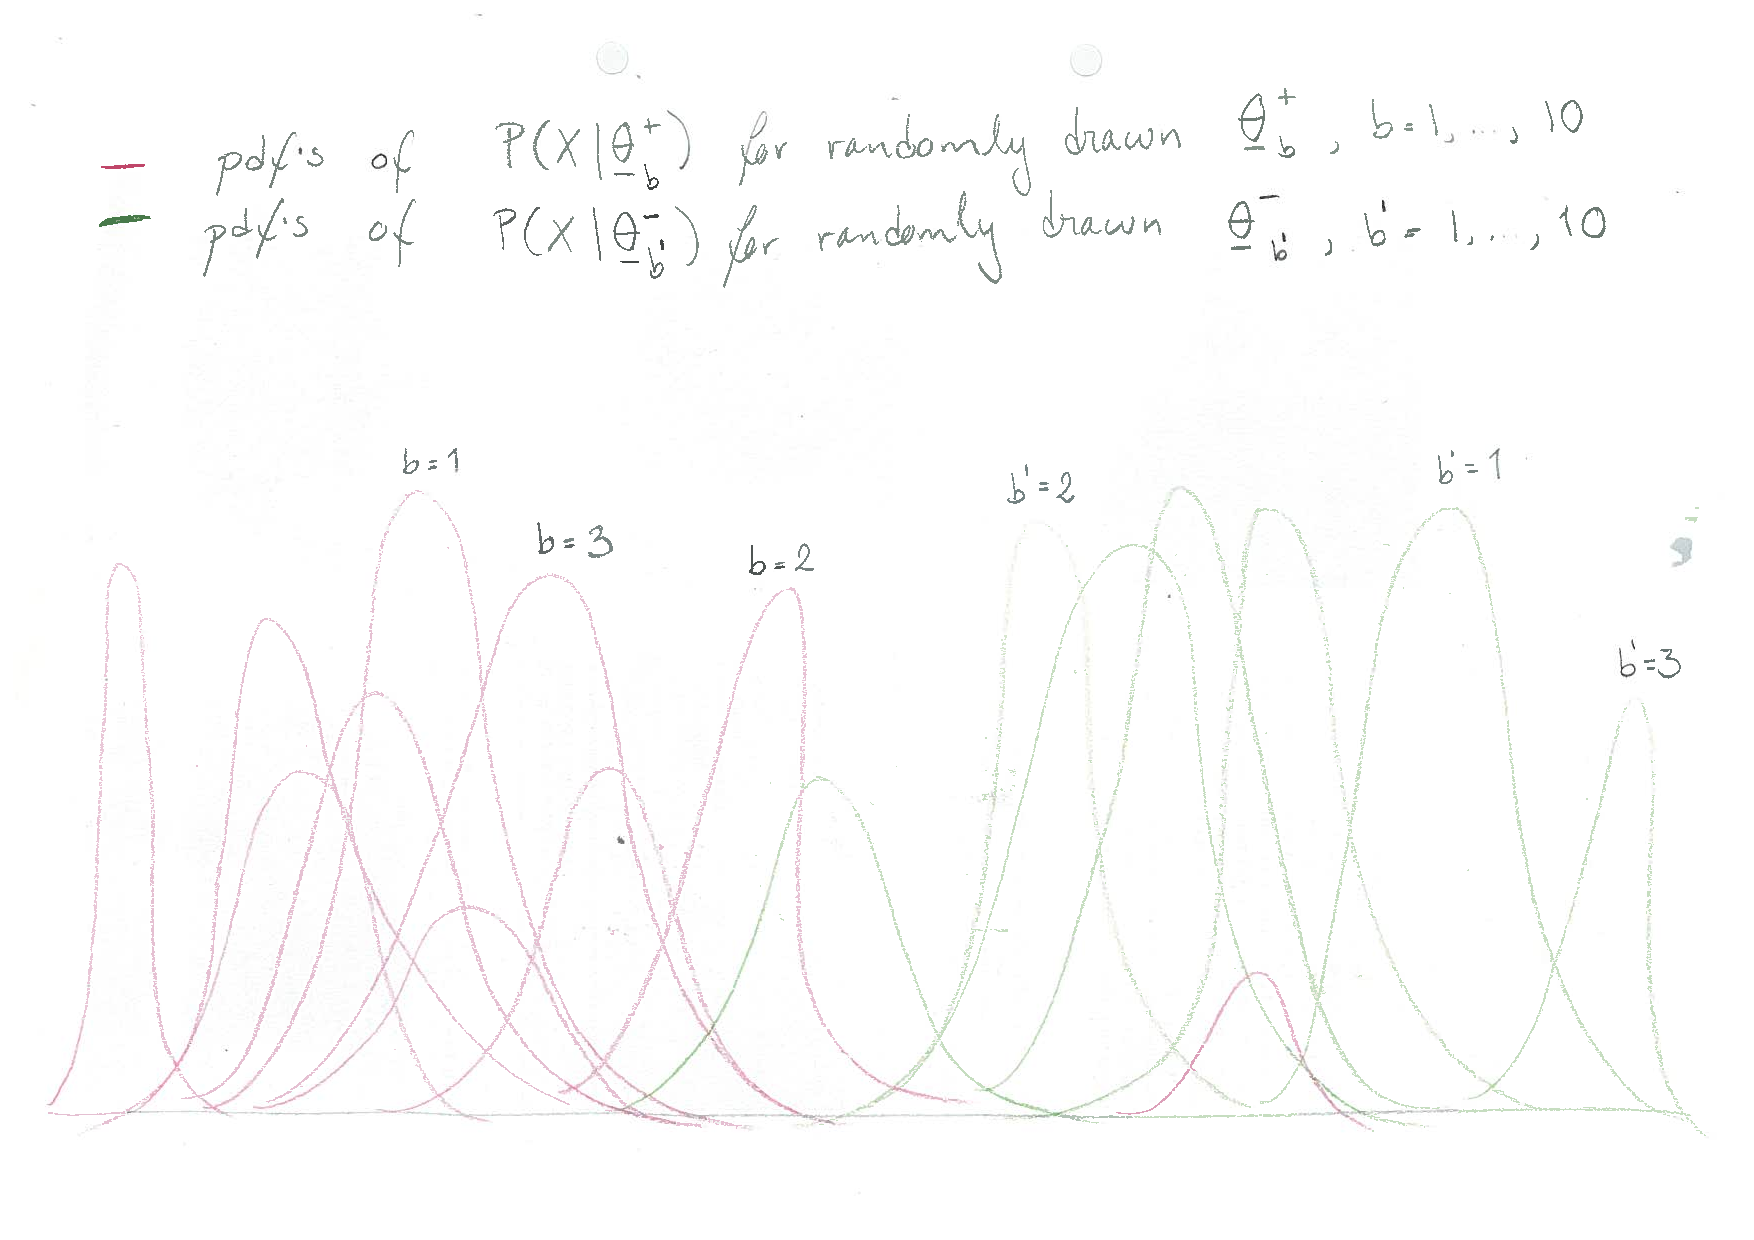
\includegraphics[height = 0.3\textheight]{Figures/distrs.pdf}
  \end{subfigure}    
  \begin{subfigure}{}
    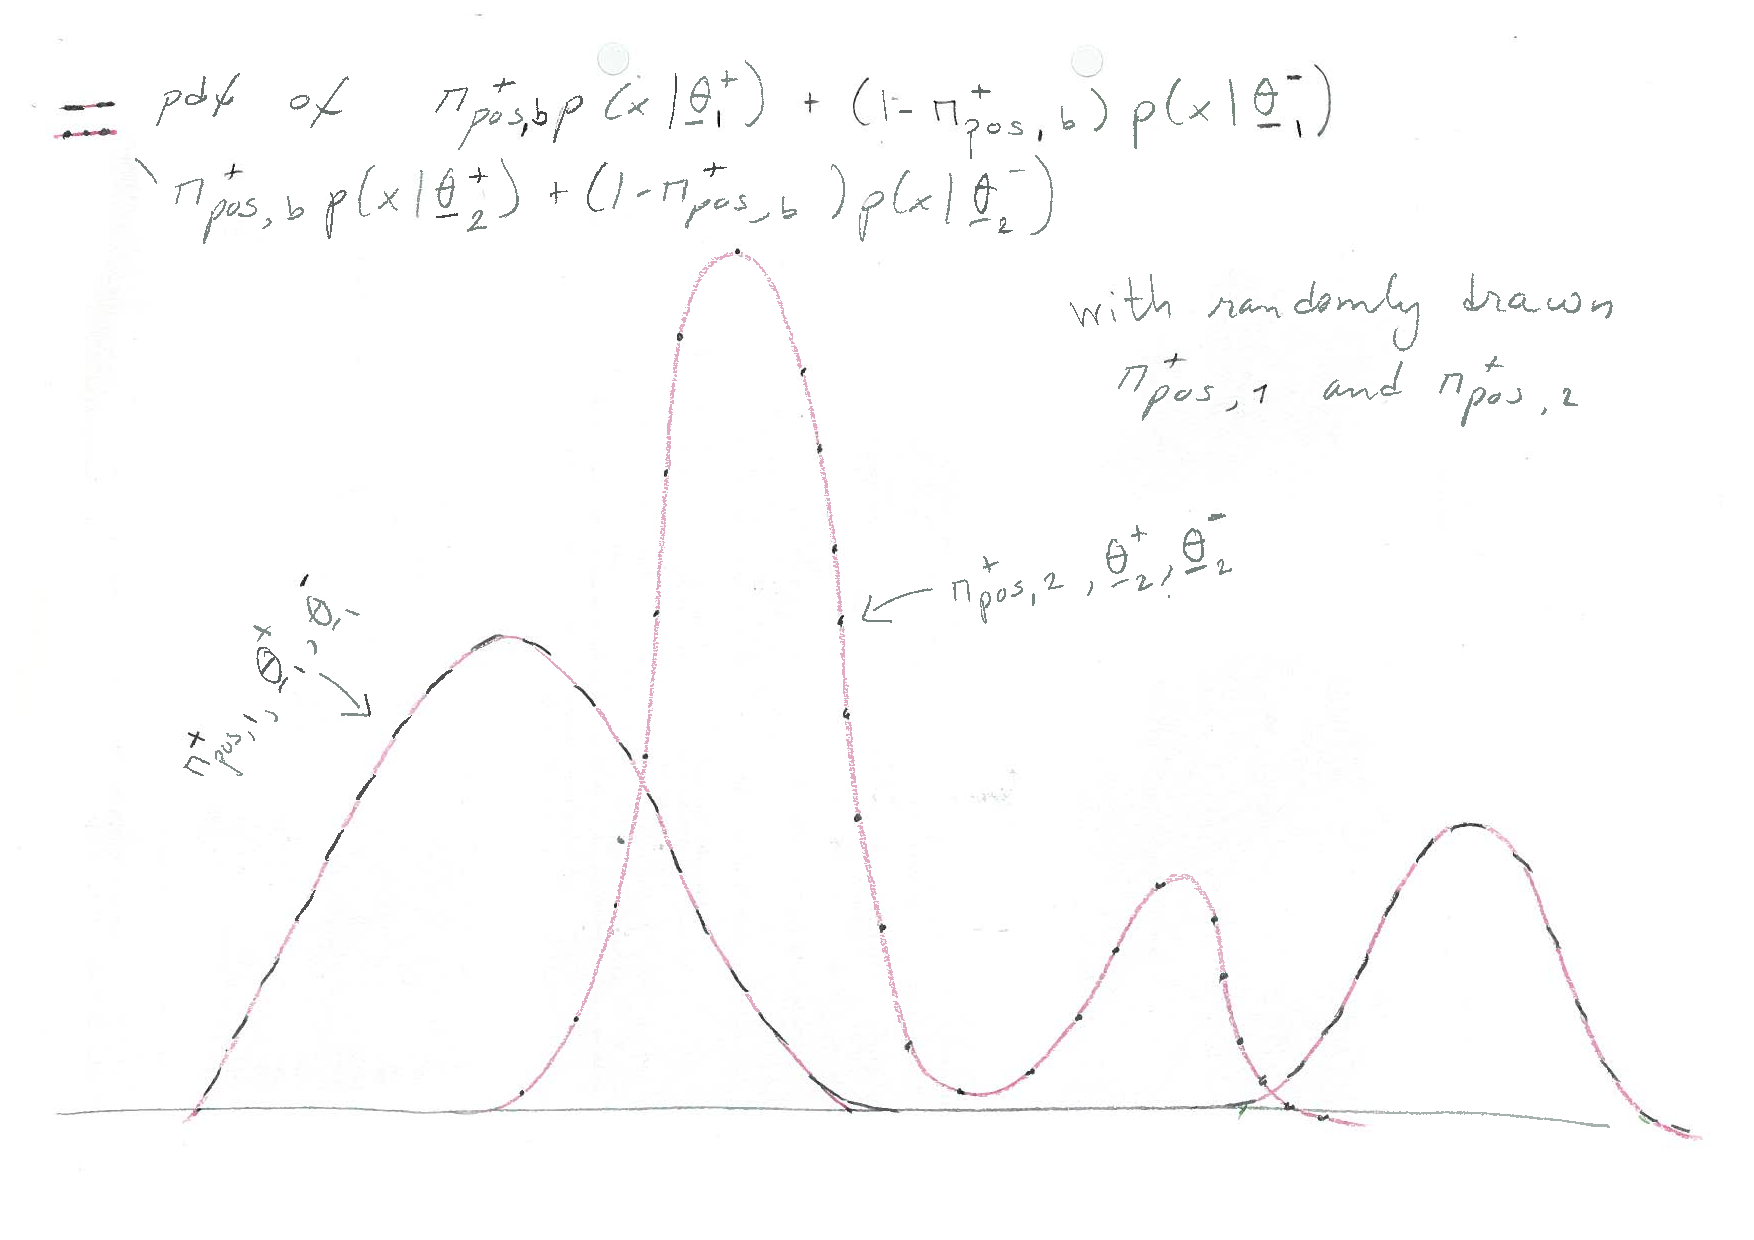
\includegraphics[height = 0.3\textheight]{Figures/pos.pdf}
  \end{subfigure}
  \begin{subfigure}{}
    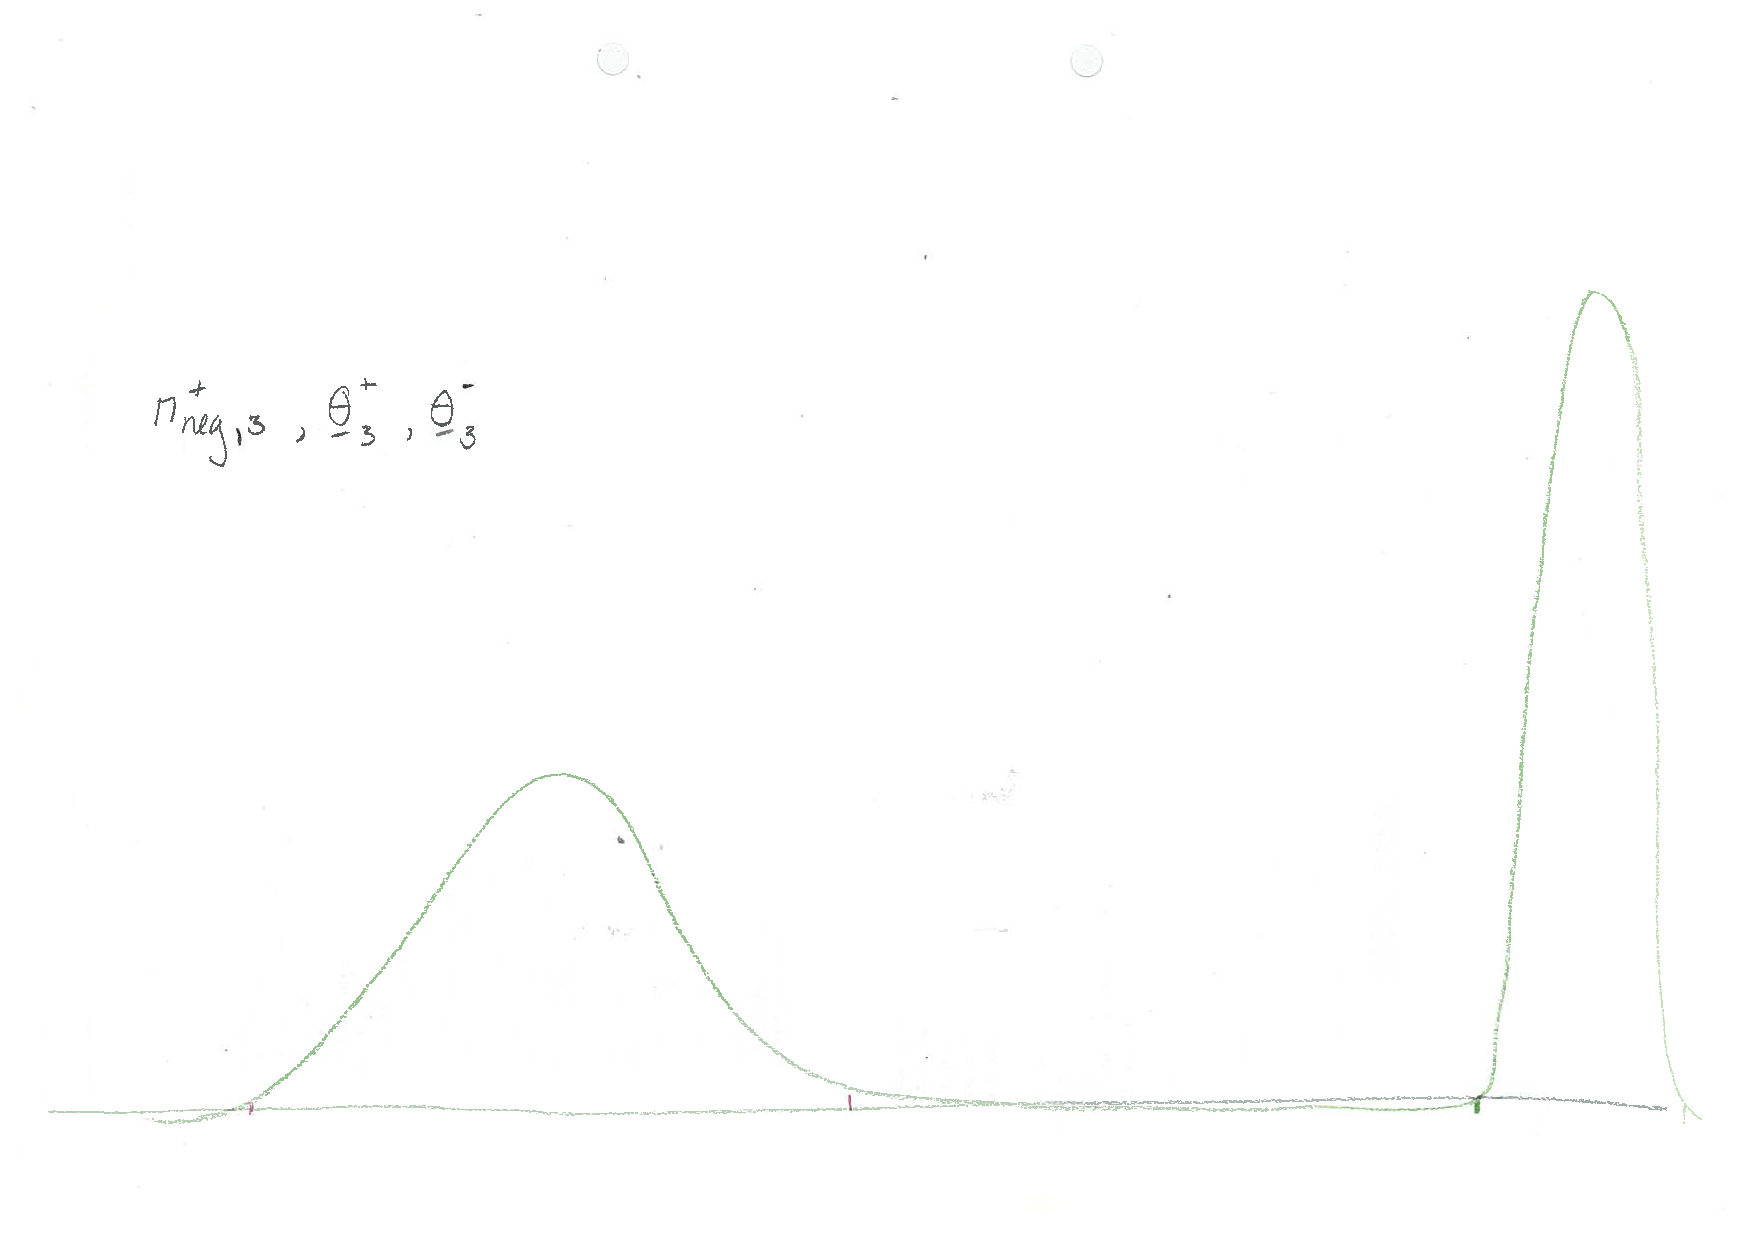
\includegraphics[height = 0.3\textheight]{Figures/neg.pdf}
  \end{subfigure}
\end{figure}

The goal is to pick a divergence that is able to discriminate between $P_{p \_ bag}$ and $P_{n \_ bag}$ by measuring the dissimilarity to $P_{pos}$ and/or $P_{neg}$.
Let $\mathcal{X}_{pos > neg}$ be the region where $p_{pos}(x) > p_{neg}(x)$. 
Unless $p_{pos} = p_{neg}$ we have $\mathcal{X}_{pos > neg}$ nonempty, which gives $\mathcal{X}_{pos < neg}$ nonempty, whereas $\mathcal{X}_{pos = neg}$ might be empty or not. 

The Kullback-Leibler information (KL inf),
\begin{align}
  d_{KL}(p_{bag},p_{neg}) = \int_\mathcal{X} p_{bag}(x) \log \frac{p_{bag}(x)}{p_{neg}(x)} dx,
\end{align}
is a non-symmetric $f$-divergence.
The log ratio function gives a positive contribution whenever $p_{bag}>p_{neg}$, and a negative contribution for $p_{bag}<p_{neg}$, and zero contribution for $p_{bag} = p_{neg}$.
A large positive contribution for $p_{bag} >> p_{neg}$ and $p_{bag} >> 0$, which means that if $p_{bag}$ is outside the range of $p_{neg}$, the dissimilarity approaches infinity. 
This is a suitable property, because if $p_{bag}/p_{neg} \rightarrow \infty$, the probability the parameters of $p_{bag}$ are not sampled from the negative class. 
A simple straightforward measure is then
\begin{align}
  D(p_{bag},p_{neg}) = d_{KL} (p_{bag},p_{neg}),
\end{align}
and the ratio $d_{KL} (p_{bag},p_{pos})/d_{KL} (p_{bag},p_{neg})$ will give a classification rule.

%We will propose a divergence-based dissimilarity function where the two classes are integrated
%\begin{align}
%  D(p_{bag},p_{neg}|p_{pos}) = \int_{\mathcal{X}_{pos}} \frac{p_{pos}(x)}{p_{neg}(x)} p_{bag}(x) \log \frac{p_{bag}(x)}{p_{neg}(x)} dx
%\end{align}
%
%{\color{red} Have a look at this
%\begin{align}
%  \int_{\mathcal{X}_{neg}} \frac{p_{pos}(x)}{p_{neg}(x)} p_{bag}(x) \log \frac{p_{bag}(x)}{p_{neg}(x)} dx \leq \geq a \int_{\mathcal{X}_{neg}} p_{bag}(x) \log \frac{p_{bag}(x)}{p_{neg}(x)} dx
%\end{align}
%}

%\begin{align}
%  D^*(p_{bag},p_{neg}|p_{pos}) = \int_{\mathcal{X}_{pos}} \frac{p_{pos}(x)}{p_{neg}(x)} p_{bag}(x) \log \frac{p_{bag}(x)}{p_{neg}(x)} dx
%						+ \int_{\mathcal{X}_{neg}} \frac{p_{pos}(x)}{p_{neg}(x)} p_{bag}(x) \log \frac{p_{bag}(x)}{p_{neg}(x)} dx
%\end{align}

Because we also assume that $\pi_{pos} > \pi_{neg}$ it follows that $p_{p \_ bag} < p_{n \_ bag}, X \in \mathcal{X}_{neg}$ and therefore 
\begin{align}
  \int_{\mathcal{X}_{neg}} \frac{p_{pos}(x)}{p_{neg}(x)} p_{p\_bag}(x) \log \frac{p_{p\_bag}(x)}{p_{neg}(x)} dx < \int_{\mathcal{X}_{neg}} \frac{p_{pos}(x)}{p_{neg}(x)} p_{n \_ bag}(x) \log \frac{p_{n \_bag}(x)}{p_{neg}(x)} dx
\end{align}
which is an unwanted property, and therefore we use only $\mathcal{X}_{pos}$.

Like with KL inf, the log ratio function ensures large positive contributions for $p_{bag} >> p_{neg}$ when also $p_{bag} >> 0$. 
In addition, we require that $p_{pos} > p_{neg}$ for this contribution to be large. 
This is because if $p_{bag} >> p_{neg}$ but $p_{pos} < p_{neg}$ we have a bag whose pdf cannot be explained by the negative class, but neither by the positive class, and therefore is uninformative for classification. 
If $p_{pos} > p_{neg}$, or even $p_{pos} >> p_{neg}$, then $D \rightarrow \infty$.
How is this different from $d_{KL}(p_{bag},p_{pos})/d_{KL}(p_{bag},p_{neg})$?
If $p_{bag}/p_{pos} \rightarrow \infty$ and $p_{bag}/p_{neg} \rightarrow \infty$, then the ratio will be one. 

Why not use bag-to-bag?

\begin{align}
  \frac{p_{bag,b}}{p_{bag,b'}} \rightarrow \infty
\end{align}




% \section{Conditional} \label{sec:Conditional}
% \begin{align}
  p_{bag(pos)} & = \pi_{pos}^+ p^+(x|\theta_b^+) + (1-\pi_{pos}^+) p^-(x|\theta_b^-) \\
  p_{bag(neg)} & = \pi_{neg}^+ p^+(x|\theta_b^+) + (1-\pi_{neg}^+) p^-(x|\theta_b^-)
\end{align}

\begin{align}
  B \rightarrow \infty : 
  \sum_{b = 1} ^B p^+(x|\theta_b^+) =  \sum_{b' = 1} ^{B'} p^+(x|\theta_{b'}^+)
\end{align}

% Not true
%\begin{align}
%  \mathcal{X}_{neg}: p_{pos} (x) < p_{neg} (x) = \sum_{b = 1} ^{B} p^-(x|\theta_{b}^-)
% \end{align}

\begin{align}
  \mathcal{X}_{neg}: p_{pos} (x) < p_{neg} (x) 
\end{align}
 
\begin{align}
  \mathcal{X}_{neg}: E(p_{bag(pos)}) < E(p_{bag(neg)})
\end{align}

\begin{align*}
  \int_{\mathcal{X}_{neg}} \frac{p_{pos}(x)}{p_{neg}(x)} p_{bag(pos)}(x) \log \frac{p_{bag(pos)}(x)}{p_{neg}(x)} dx <
   \int_{\mathcal{X}_{neg}} \frac{p_{pos}(x)}{p_{neg}(x)} p_{bag(neg)}(x) \log \frac{p_{bag(neg)}(x)}{p_{neg}(x)} dx
\end{align*}
 

% \section{Bag-to-class} \label{sec:Bag_vs_Class}
% Why not use bag-to-bag?

\begin{align}
  \frac{p_{bag,b}}{p_{bag,b'}} \rightarrow \infty
\end{align}

% \section{Non-hierarchical model} \label{sec:Non_Hierarchical}
% The positive instances are observations from $p^+(x|\theta^+)$. 
The negative instances are observations from $p^-(x|\theta^-)$. 
A positive bag contains the observations:
\begin{align}
  p_{bag(pos)}(x) = \pi_{pos}^+ p^+(x|\theta^+) + (1-\pi_{pos}^+) p^-(x|\theta^-)
\end{align}
A negative bag contains the observations:
\begin{align}
  p_{bag(neg)}(x) = \pi_{neg}^+ p^+(x|\theta^+) + (1-\pi_{neg}^+) p^-(x|\theta^-)
\end{align}

If all positive bags follow the same distribution and all negative bags follow the same distribution, then the best estimation of $p_{bag(pos)}(x)$ is to pool all instances from the positive bags, and we get $\hat{p}_{bag(pos)}(x)$.
We can then look at $\hat{p}_{bag(pos)}(x)$ and $\hat{p}_{bag(neg)}(x)$ as prototypes to which the distance from $\hat{p}_{bag}(x)$ is measured.

However, more realistically, we assume that 
\begin{align}
  p_{bag(pos),b}(x) = \pi_{pos,b}^+ p^+(x|\theta^+_b) + (1-\pi_{pos,b}^+) p^-(x|\theta^-_b)
\end{align}
and that 
\begin{align}
  p_{pos}(x) = \sum_{b=1}^B p_{bag(pos),b}(x) = \sum_{b=1}^B \pi_{pos,b}^+ p^+(x|\theta^+_b) + (1-\pi_{pos,b}^+) p^-(x|\theta^-_b)
\end{align}

%Since $n_{bag} << n_{pos} \approx n_{neg}$, $D(\hat{p}_{bag}, p_{neg}) > D(\hat{p}_{neg}, p_{neg})$, and we cannot expect $D(\hat{p}_{bag(neg)},\hat{p}_{neg}) \approx \min(D)$.

Assume that $\pi_{pos}^+ p^+(x|\theta^+)$ to $\pi_{neg}^+ p^+(x|\theta^+)$ is more discriminative than $(1-\pi_{pos}^+) p^-(x|\theta^-)$
to $(1-\pi_{neg}^+) p^-(x|\theta^-)$. 
% In addition $\pi_{pos}^+ < 0.5$.
% In other words, the positive instances are few, but have more discriminative power than the negative instances. 
\begin{align}
  \frac{\pi_{pos}^+}{\pi_{neg}^+} > \frac{1-\pi_{pos}^+}{1-\pi_{neg}^+} 
\end{align}
% The same distortion in $\hat{f}^+$ as in $\hat{f}^-$ will lead to a greater non-overlapping area at $\hat{f}^-$
Therefore, non-symmetric divergence function. 
Kullback-Leibler meets the requirement.

% section{Bayes hierarchy} \label{sec:Bayes_hierarchy}
% A random variable $X_{pos}$ from a positive bag can be seen as a three level Bayes hierarchy. $X_{pos}$ is distributed with parameter $\theta$, which is a random variable. $\theta$ is distributed with parameter $\tau$, which takes value $\tau^+$ with probability $p = \pi_{pos}^+$ and $\tau^-$ with probability $p = 1-\pi_{pos}^+$.
\begin{align}
  X_{pos}|\theta & \sim P(X_{pos} | \theta) \\
  \theta|\tau &  \sim P(\theta|\tau) \\
  \tau & \sim \begin{cases}
    \tau^+, & \text{with probability } p = \pi_{pos}^+\\
    \tau^-, & \text{with probability } p = 1-\pi_{pos}^+
  \end{cases}
\end{align}

The pdf of the $b$th positive bag is then
\begin{align}
  f_{b,pos}(x) = \pi_{pos}^+ f^+(x|\theta^+_b) +(1-\pi_{pos}^+) f^-(x|\theta^-_b), 
\end{align}
where $\theta^+_b$ is the $b$th observation of the random variable $\theta$ with parameter $\tau^+$, and $\theta_b^-$ is the $b$th observation of the random variable $\theta$ with the parameter $\tau^-$.
The pdf of positive bags is then
\begin{align*}
  f_{pos}(x) = \pi_{pos}^+ \int_{\Theta|\tau^+} f^+(x|\theta)h(\theta|\tau^+) d\theta|\tau^+  +(1-\pi_{pos}^+) \int_{\Theta|\tau^-} f^-(x|\theta) h(\theta|\tau^-) d\theta|\tau^-, 
\end{align*}
where $\theta^+_b$ is the $b$th observation of the random variable $\theta$ with parameter $\tau^+$, and $\theta_b^-$ is the $b$th observation of the random variable $\theta$ with the parameter $\tau^-$.

Similarly for negative bags we have
\begin{align}
  X_{neg}|\theta & \sim P(X_{neg} | \Theta) \\
  \Theta|\mathcal{T} &  \sim P(\theta|\tau) \\
  \tau & \sim \begin{cases}
    P(\mathcal{T} = \tau^+) = \pi_{neg}^+\\
    P(\mathcal{T} = \tau^-  = 1-\pi_{neg}^+
  \end{cases}
\end{align}
and
\begin{align}
  f_{{b'},neg}(x) = \pi_{neg}^+ f^+(x|\theta^+_{b'}) +(1-\pi_{neg}^+) f^-(x|\theta^-_{b'}), 
\end{align}

\section{Equality and orthogonality} \label{sec:Eq_Orth}
\begin{enumerate}
  \item $f_{bag}(x) = f_{NEG}(x)$
  \item $f_{bag}(x) = f_{POS}(x)$
  \item $f_{\cpos}(x) = f_{NEG}(x)$
  \item $f_{bag}(x) \perp f_{NEG}(x)$
  \item $f_{bag}(x) \perp f_{POS}(x)$
  \item $f_{POS}(x) \perp f_{NEG}(x)$
\end{enumerate}
$condI_{KL}(bag,\cneg|\cpos) = \int_{\mathcal{X}_{POS}} \frac{f_{POS}(x)}{f_{NEG}(x)} f_{bag}(x) \log \frac{f_{bag}(x)}{f_{NEG}(x)} dx$ 
\begin{enumerate}
  \item $ \int_{\mathcal{X}_{POS}} \frac{f_{POS}(x)}{f_{NEG}(x)} f_{NEG}(x) \log \frac{f_{NEG}(x)}{f_{NEG}(x)} dx = 0$ 
  \item $\int_{\mathcal{X}_{POS}} \frac{f_{POS}(x)}{f_{NEG}(x)} f_{POS}(x) \log \frac{f_{POS}(x)}{f_{NEG}(x)} dx$ 
  \item $\int_{\mathcal{X}} f_{bag}(x) \log \frac{f_{bag}(x)}{f_{NEG}(x)} dx$ 
  \item $\int_{\mathcal{X}_{POS}} \frac{f_{POS}(x)}{f_{NEG}(x)} f_{bag}(x) \log \frac{f_{bag}(x)}{f_{NEG}(x)} dx = \infty$ 
  \item $\int_{\mathcal{X}_{POS}} \frac{f_{POS}(x)}{f_{NEG}(x)} f_{bag}(x) \log \frac{f_{bag}(x)}{f_{NEG}(x)} dx = 0$ 
  \item $\int_{\mathcal{X}_{POS}} \frac{f_{POS}(x)}{f_{NEG}(x)} f_{bag}(x) \log \frac{f_{bag}(x)}{f_{NEG}(x)} dx = \infty$ 
\end{enumerate}
$D_{KL} = \int f_{bag}(x) \log \frac{f_{bag}(x)}{f_{NEG}(x)} dx / \int f_{bag}(x) \log \frac{f_{bag}(x)}{f_{POS}(x)} dx$
\begin{enumerate}
  \item $\int f_{NEG}(x) \log \frac{f_{NEG}(x)}{f_{NEG}(x)} dx / \int f_{NEG}(x) \log \frac{f_{NEG}(x)}{f_{POS}(x)} dx = 0$
  \item $ \int f_{POS}(x) \log \frac{f_{POS}(x)}{f_{NEG}(x)} dx / \int f_{POS}(x) \log \frac{f_{POS}(x)}{f_{POS}(x)} dx = \infty$
  \item $\int f_{bag}(x) \log \frac{f_{bag}(x)}{f_{NEG}(x)} dx / \int f_{bag}(x) \log \frac{f_{bag}(x)}{f_{NEG}(x)} dx = 1$
  \item $\int f_{bag}(x) \log \frac{f_{bag}(x)}{f_{NEG}(x)} dx / \int f_{bag}(x) \log \frac{f_{bag}(x)}{f_{POS}(x)} dx = \infty$
  \item $\int f_{bag}(x) \log \frac{f_{bag}(x)}{f_{NEG}(x)} dx / \int f_{bag}(x) \log \frac{f_{bag}(x)}{f_{POS}(x)} dx = 0$
  \item $\int f_{bag}(x) \log \frac{f_{bag}(x)}{f_{NEG}(x)} dx / \int f_{bag}(x) \log \frac{f_{bag}(x)}{f_{POS}(x)} dx$\end{enumerate}

% \section{Regions} \label{sec:Regions}
% \noindent$
condI_{KL}(bag,\cneg|\cpos) \\
\mathcal{X}_{POS} : condI_{KL} (bag(\cpos)) > condI_{KL} (bag(\cneg))\\
\mathcal{X}_{NEG} : condI_{KL} (bag(\cpos)) < condI_{KL} (bag(\cneg))\\
$
\begin{align}
& D_{KL}(\frac{bag,\cpos}{bag,\cneg})\\
\mathcal{X}_{\cpos} & : I_{KL}(bag(\cpos),\cpos) > I_{KL}(bag(\cneg),\cpos) \\
& : I_{KL}(bag(\cpos),\cneg) > I_{KL}(bag(\cneg),\cneg) \\
& D_{KL} ? \\
\mathcal{X}_{\cneg} & : \text{similar} 
\end{align}

\clearpage
\section{Nomenclature} \label{sec:Nomenclature}
\begin{align*}
  f(x) : & \text{ probability density function (pdf)} \\
  f^+(x) : & \text{ pdf of positive instances} \\
  f^-(x) : & \text{ pdf of negative instances} \\
  f_{bag}(x) : & \text{ pdf of bag (unknown class)} \\
  f_{pos}(x) : & \text{ pdf of positive bag} \\
  f_{neg}(x) : & \text{ pdf of negative bag} \\
  f_{POS} (x) : & \text{ pdf of positive labelled bags} \\
  f_{NEG} (x) : & \text{ pdf of negative labelled bags} \\
  \Pi_{pos}^+ : & \text{ probability of an instance in a positive bag being sampled for } f^+(x)\\
  \Pi_{neg}^+ : & \text{ probability of an instance in a negative bag being sampled for } f^+(x) \\
  X_{pos} : & \text{ random variabel in positive bag} \\
  x_{pos,b,i} : & \text{ observation $i$ in positive bag $b$} \\
  X_{neg} : & \text{ random variabel in negative bag} \\
  x_{neg,{b'},i} : & \text{ observation $i$ in negative bag $b'$} \\
  \Theta^+ : & \text{ random variable with distribution parameter } \tau^+ \\
  \theta_b^+ : & \text{ $b$th distribution parameter (observation of $\Theta^+$)} \\
  \Theta^- : & \text{ random variable with distribution parameter $\tau^-$} \\
  \theta_b^- : & \text{ $b$th distribution parameter (observation of $\Theta^-$)} \\
  \mathcal{T} : & \text{ random variable} \\
  \tau^+, \tau^- : & \text{ observations of $\mathcal{T}$} \\
\end{align*}
 

\section{Notes} \label{sec:Notes}
(3) Conditional divergence

Concept: Automatically identifies the concept(s) as $x \in \mathcal{X}: f_{pos} > f_{neg}$

``Point set distance measures''

Strong class overlap

Assumptions?\\
\begin{align}
  \frac{\pi_{pos}^+}{\pi_{neg}^+} & \text{ vs } \frac{a-\pi_{pos}^+}{1-\pi_{neg}^+} \\
  \theta^+ & \text{ vs } \theta^-
\end{align}

Class level: Good density estimates\\
High dimensions: Assume independence

\subsection{Kullback-Leibler} 

$f_{bag} \perp f_{neg} : D_{KL} = \infty$ contribution \\
Conditional: $f_{bag} \perp f_{neg}$ and in addition $f_{bag} \perp f_{pos} : D_{KL|pos} = 0$ contribution

\begin{itemize}
  \item Drawback: Not for one-vs-all. Solution: Well-defined classes (sea, sand, desert)
  \item Other: Multi-label learning, regression, clustering, semi-supervised
  \item Kernel density estimation
  \item No estimation of weight
  \item Drawback of classical CBIR
\end{itemize}


%% Bibliography
\bibliographystyle{elsarticle-num} 
\bibliography{/Users/kam025/kajsam}

\end{document}
